\section{Task 2}



\begin{lstlisting}
typedef struct Cell
{
	uint8_t direction[MAX_PLAYER_COUNT];
	uint16_t neighbor[MAX_PLAYER_COUNT];
} Cell;


class Map
{
	private:
		uint16_t overrideStones[MAX_PLAYER_COUNT];
		uint16_t numberOfBombes[MAX_PLAYER_COUNT];
		uint8_t playerMap[MAX_PLAYER_COUNT + 1];
			// 0xFF means the player is not playing. playerMap[0] is also a player not playing.
		
		void addNeighbour(uint32_t x1, uint32_t y1, uint8_t dir1, uint32_t x2, uint32_t y2, uint8_t dir2);

	public:
		char* board;
	
		Map(std::string path);
		Map(Map& toCopyMap);
		virtual ~Map();
		Cell getCell(uint8_t x, uint8_t y);
		void draw();
		bool isMoveValid(uint8_t x, uint8_t y, uint8_t player, uint8_t information);
		int32_t evaluateForPlayingPhase(uint8_t player);
		int32_t evaluateForBombingPhase(uint8_t player);

};
\end{lstlisting}
\newpage
In the first stage of the creation of the data structure, we parse the map to a two dimensional array and count the number of occupied cells. We need this number to create array of the according size and as we are already reading the map in, we save it in a more handy format.\\
In the next stages of loading the map, we split the information into a static part, which will remain unchanged during a game, and a dynamic part. To anticipate a lot of map copying to evaluate different possible moves, we did try to reduce the size of the dynamic part as much as possible.\\\\

The data structure we came up with consists of 3 parts, which are best explained with the help of an example. For latter we take the following four by four board:\\
$
\addvbuffer[20pt 20pt]{
\begin{tabular}{*{4}{|z{2.5em}}|}
	\hline
	- & - & - & -\\
	\hline
	- & 1 & 2 & 0\\
	\hline
	- & b & - & 0\\
	\hline
	0 & 0 & 0 & c\\
	\hline
\end{tabular} }
$

We begin by copying the states off every cell into an one dimensional array (\textbf{board}). This array is the only dynamic part, because it saves all the information that can change during a game. As it has a size of only $width * height$ bytes, the copying of a lot of boards to execute different moves should be as fast as possible.

$
\addvbuffer[20pt 20pt]{
\begin{tabular}{*{9}{|z{2.5em}}|}
\hline
1 & 2 & 0 & b & 0 & 0 & 0 & 0 & c\\
\hline
\end{tabular}}
$

The second thing we do is to create our \textbf{offsetMap}. That is an two by two array off the same size as the initial board. In that array we save, for every cell, how many cells exist before it, while ignoring the holes. On the positions of holes, we simply write a $-1$.

$
\addvbuffer[25pt 25pt]{
\begin{tabular}{*{4}{|z{2.5em}}|}
	\hline
	-1 & -1 & -1 & -1\\
	\hline
	-1 & 0 & 1 & 2\\
	\hline
	-1 & 3 & -1 & 4\\
	\hline
	 5 & 6 & 7 & 8\\
	 \hline
\end{tabular}}
$

Finally, we need to save how all the cells are linked together. To archive this, we created a struct \textbf{Cell}, which consists of two arrays, \textbf{neighbour} and \textbf{direction}, each with an entry for every possible direction.\\

\textbf{neighbour[}direction\textbf{]} saves the index of the neighbour in that that direction. Here again, we write an -1 if in a specific direction the cell borders no other cell.\\

As we can change the direction of a line throw artificially added transitions,\\ \textbf{direction[}direction\textbf{]} saves the direction in which the map traversing algorithm has to continue looking. 

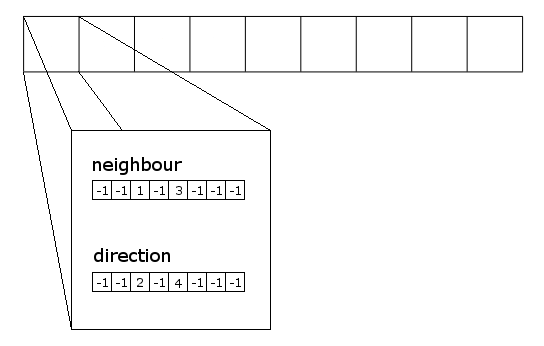
\includegraphics[width=14cm, height=8cm]{datastructure.png}

